\documentclass[a4paper,12pt]{article}
\usepackage{cmap}
\usepackage[T1,T2A]{fontenc}  % кодировка
\usepackage[utf8]{inputenc}   % кодировка исходного текста
\usepackage[english,russian]{babel} % локализация и переносы
\usepackage{geometry}
\usepackage{titling}
\usepackage{minted}
\usepackage{graphics}
\usepackage{graphicx}

\renewcommand\maketitlehooka{\null\mbox{}\vfill}
\renewcommand\maketitlehookd{\vfill\null}


% геометрия
\geometry{pdftex, left = 2cm, right = 2cm, top = 2.5cm, bottom = 2.5cm}
\setcounter{tocdepth}{4} % фикс переноса 
\righthyphenmin = 2
\tolerance = 2048

% заголовок
\title{Отчет по Лабораторной работе №9\\[150mm]}
\author{Чепиго Дарья \\ИУ7-44Б}
\date{}



\begin{document}
	\begin{titlepage}
		\maketitle
		\thispagestyle{empty}
	\end{titlepage}
	
	\newpage
	\noindent\textbf{Условие задачи:}
	
	Реализация и исследование олгоритма Сазерленда-Ходжмена отсечения многоугольников.\\
	
	\noindent\textbf{Этапы работы программы:}
	\begin{enumerate} 
		\item Ввод отсекателя
		\item Ввод многоугольника
		\item Выполнение отсечения: границы отсекателя показать одним цветом, отрезок -- другим, результат отсечения -- третьим.
	\end{enumerate}
	""

	\noindent\textbf{Алгоритм Сазерленда-Ходжмена:}

	Алгоритм Сазерленда-Ходжмена позволяет выпуклым отсекателем отсечь многоугольник. Плоский многоугольник - часть плоскости, ограниченная замкнутой плоской линией(при отсечении результат может включать ребра отсекателя).\\
	
	Идея алгоритма - решение задачи последовательно: многоугольник отсекается относительно каждой грани отсекателя по отдельности и при этом результат, полученный на i-ом шаге служит исходным для i+1-ого отсечения.\\
	
	
	Для отсечения нужно определять принадлежность точки рассматриваемого многоугольника плоскости отсекателя относительно очередной грани.\\

	Это решается с помощью векторного произведения и алгоритма из прошлой лабораторной работы. Если векторное произведение в правовинтовой (вершины рассматриваются против часовой стрелки) системе < 0, то вершина лежит вне плоскости отсекателя, иначе - внутри (относительно рассматриваемой на данный момент грани).\\
	\newpage
	В процессе рассмотрения ребер отсекаемого многоугольника возможны следующие положения (направление ребра от вершины P к вершине S; параллельные линии без стрелочек - область отсекателя):\\
	
	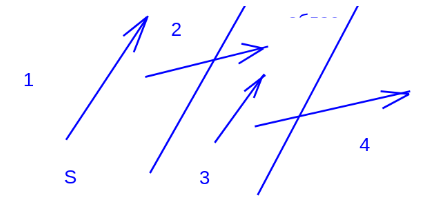
\includegraphics[width=\linewidth]{lines}
	
	\begin{enumerate} 
		\item Ребро полностью вне рассматриваемой границы отсекателя. В таком случае не добавляем никакую вершину.
		\item Ребро пересекает границу отсекателя, причем вершина S - внутри, а Р - нет. В таком случае нужно добавить в список вершин искомого отсеченного многоугольника вершину S, а так же точку пересечения текущего ребра с рассматириваемой гранью.
		\item Ребро полностью находится внутри отсекателя. В таком случае следует добавить обе вершины в список вершин искомого многоугольника.
		\item Ребро пересекает границу отсекателя, причем вершина S - вне отсекателя, а Р - внутри. В таком случае нужно добавить в список вершин искомого отсеченного многоугольника вершину Р, а так же точку пересечения текущего ребра с рассматириваемой гранью.
	\end{enumerate}
	""
	
	Пересечение в данном алгоритме я находила так же, как в алгоритме Кируса-Бека: имеется
	\begin{enumerate} 
		\item вектор внутренней нормали
		\item отрезок (заданный двумя точками, очередное ребро отсекаемого многоугольника)
		\item грань (тоже задана 2 точками, вершинами отсекателя)
	\end{enumerate}
	\newpage
	Находим d - вектор ориентации ребра многоугольника, wi - вектор, соединяющий точку грани (первую для определенности), а также скалярные произведения 
	\[Wck = (n, wi)\]
	\[Dck = (d, n)\]
	 где n - вектор внутренней нормали.\\
	Далее найдем параметр t \[t = -Wck / Dck\]
	он точно будет в [0, 1] и выразим Х, У точки пересечения:
	
	\[X = P1.x + (P2.x - P1.x) * t\]
	\[Y = P1.y + (P2.y - P1.y) * t\]
	
	В целом алгоритм очень похож на алгоритм Кируса-Бека, поэтому в данном отчёте не такое большое описание происходящего.
	
	\newpage
	\noindent\textbf{Алгоритм с комментариями из моей программы (файл main.py):}
	\begin{minted}[fontsize=\footnotesize]{python3}
	def sazerland_hodjmen_alg():
	cutter = wind.cutter
	polygon = wind.polygon
	
	# Проверка на замкнутость полигона
	if not end_polygon_:
		end_polygon()
	
	add_polygon(cutter, wind.pen_cutter)
	
	count_sides = len(cutter)
	
	# Цикл по сторонам отсекателя
	for i in range(-2, count_sides  - 2):
		# Вычисление вектора внутренней нормали к очередной
		# i-ой стороне отсекателя - N_вi
		norm = normal(cutter[i], cutter[i + 1], cutter[i + 2])
		# полигон, отсеченный текущей стороной
		cutted_polygon = []
	
		# цикл по сторонам полигона
		for j in range(-1, len(polygon) - 1):
			p1, p2 = polygon[j], polygon[j + 1]
			# Вычисление вектора W_i=P_1-f_i (f_i берем за вершины стороны)
			w1 = [p1.x() - cutter[i].x(), p1.y() - cutter[i].y()]
			w2 = [p2.x() - cutter[i].x(), p2.y() - cutter[i].y()]
	
			w1_scal = scalar_mult(w1, norm)
			w2_scal = scalar_mult(w2, norm)
			
			if w1_scal < 0 and w2_scal < 0:
			#  отрезок вне видимой области
				continue
			elif w1_scal > 0 and w2_scal > 0:
				# отрезок полностью в видимой области
				# p1 была занесена в результат на предыдущем шаге
				cutted_polygon.append(p2)
				continue
				
		# отрезок пересекает сторону отсекателя
		
		# Вычисление директрисы отрезка:
		# D = P_2-P_1
		d = [p2.x() - p1.x(), p2.y() - p1.y()]
		
		d_scal = scalar_mult(d, norm)
		if d_scal == 0:
			if w2_scal < 0:
				cutted_polygon.append(p2)
			continue
	
		# Находим коэф пересечения.
		t = -w1_scal / d_scal
		# Точка пересечения
		pt = QPoint(round(lerp(p1.x(), p2.x(), t)),
			round(lerp(p1.y(), p2.y(), t)))
		
		if w1_scal < 0:
		# отрезок направлен в сторону внутренней области отсекателя
			cutted_polygon.append(pt)
			cutted_polygon.append(p2)
		else:
			# отрезок направлен от внутренней области отсекателя
			# p1 была занесена в результат на предыдущем шаге
			cutted_polygon.append(pt)
		
	polygon = cutted_polygon
	
	add_polygon(polygon, wind.pen_res)
	\end{minted}


	\newpage
	\noindent\textbf{Интерфейс и примеры работы:}\\\\
	Главное окно и невыпуклый отсекатель:\\\\
	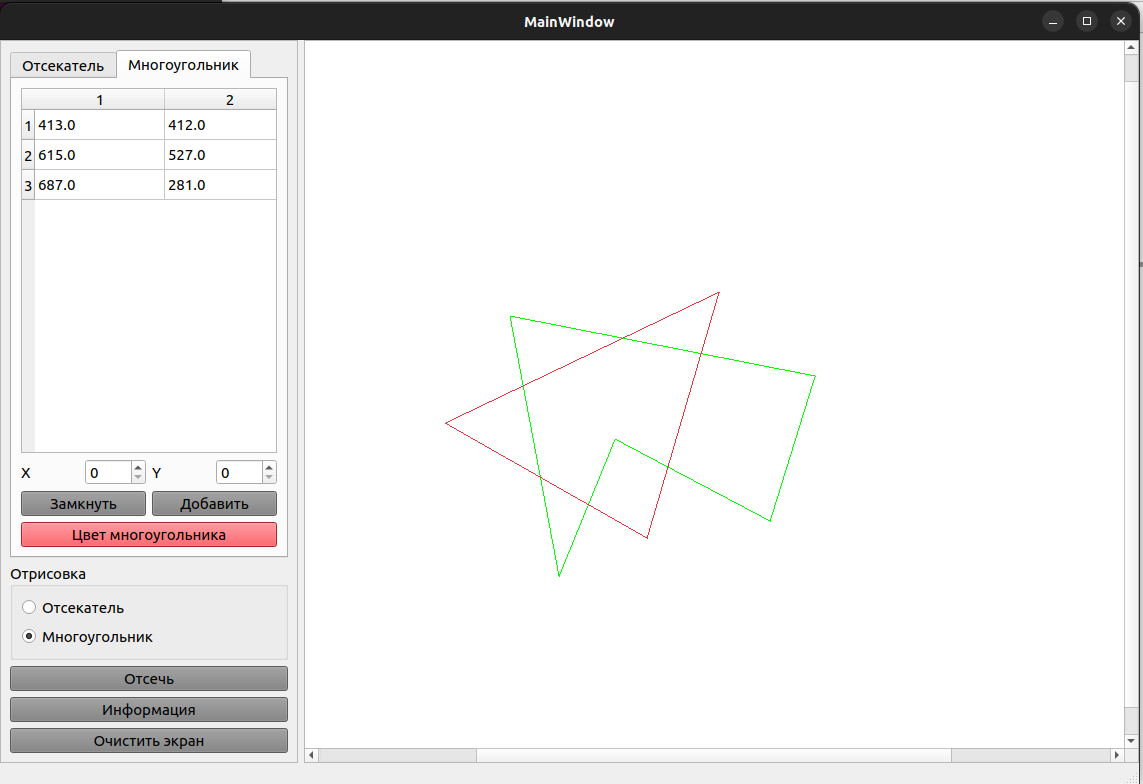
\includegraphics[width=\linewidth]{mainwin}\\\\
	Информация о программе:\\\\
	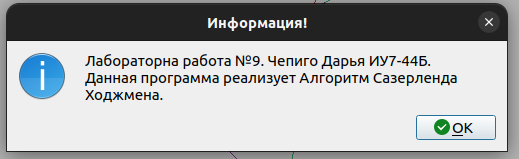
\includegraphics[width=\linewidth]{infor}
	\newpage
	Меняем цвет:\\\\
	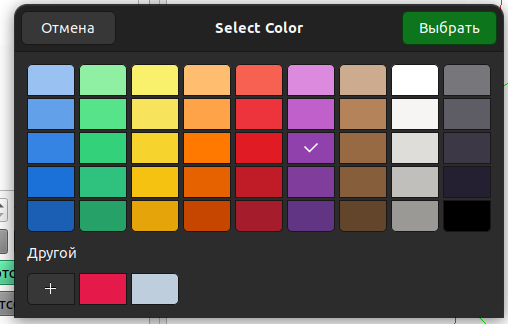
\includegraphics[width=\linewidth]{color}\\
	\noindent Попробуем отсечь:\\\\
	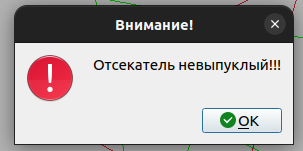
\includegraphics[width=\linewidth]{errorpol}\\\\
	\newpage
	\noindent Зададим выпуклый отсекатель и отрезки, выберем цвет отсекаемых отрезков:\\
	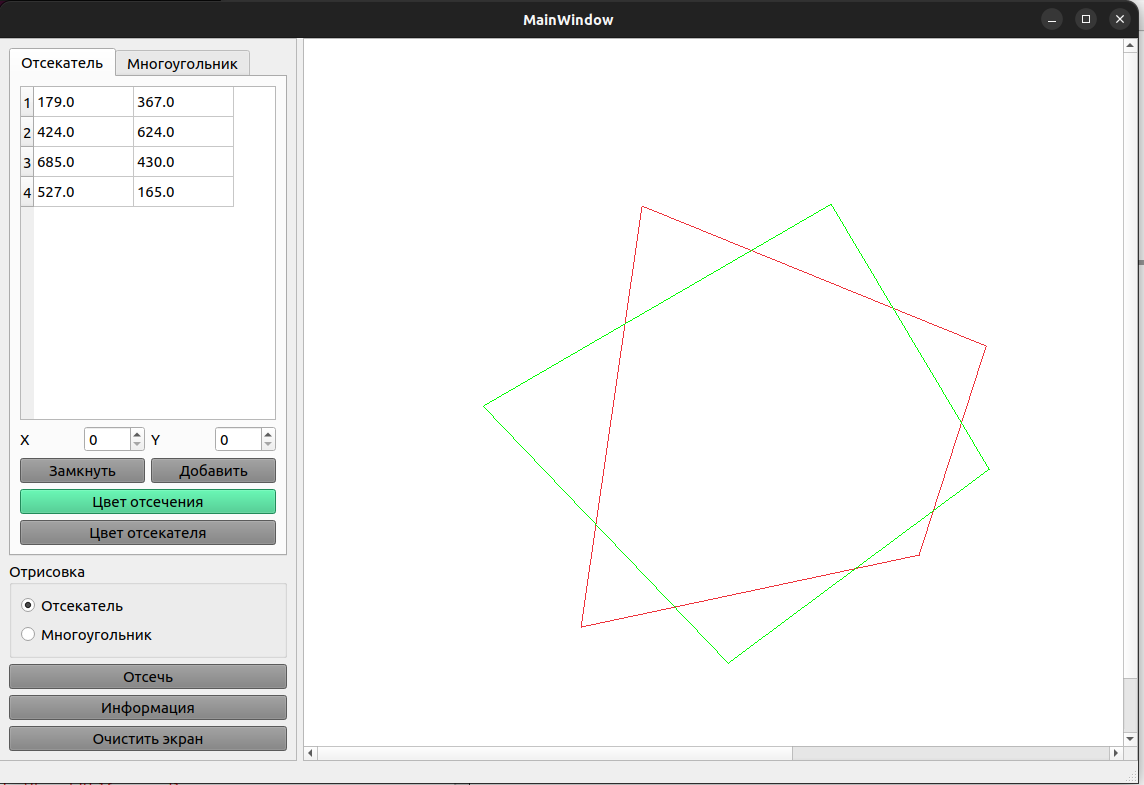
\includegraphics[width=\linewidth]{normalpol}\\
	отсекаем:\\
	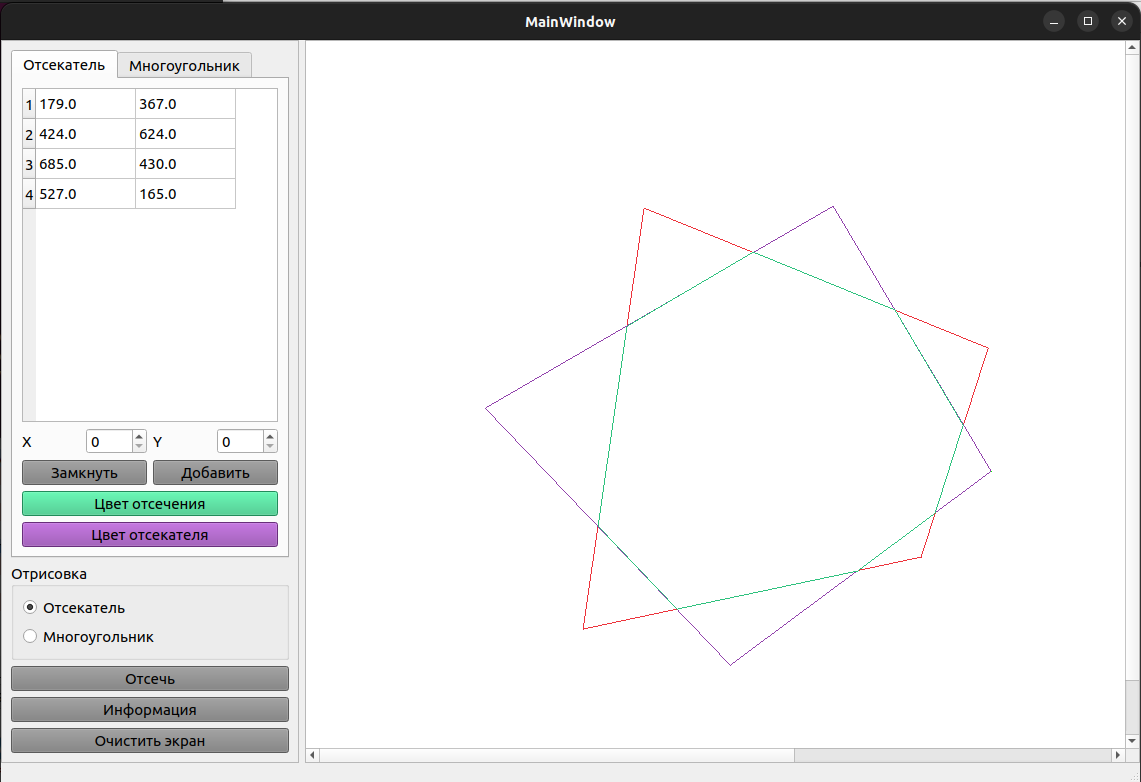
\includegraphics[width=\linewidth]{res}

\end{document}